\Chapter{Koncepció}

\Section{A fejezet célja}

A szimulációs környezet inspirációt vesz már elkészített szimulációokból, mint például a Pixel Dungeon \cite{pixeldungeon} és Darkest Dungeon \cite{darkestdungeon} 
nevű játékokból ismerhető szoba és folyosó kapcsolat. Ahol minden szobát egy folyosó köt össze egy másik tetszőleges szobával.
A Darkest Dungeon-hoz képest a játékmenet rugalmasabb, mivel a szobák bármikor elhagyhatóak és megközelíthetőek, ha engedi azt a pálya jelenlegi belső felépítése.
Azaz, ha nincs útban valami, ami megakadályozza.

A fent említett két játék mind körökre osztott, ahogyan a szimulációs környezetünk is az lesz.

A szimulációs környezetünk viszont egyedi lesz abból a szempontból, hogy az ágensek csoportokra vannak osztva és közös céllal
rendelkezve próbálják legyőzni egymást és az ellenséges ágenseket.

\Section{Felhasznált technológiák}

\noindent Pixel Dungeon:

\begin{itemize}
    \item Körökre osztott tevékenységkör.
    \item A játék szobák és folyosók véges kombinációjából épül fel.
    \item A játéktér teljes része négyzet cellákból épül fel, amelyek összességét.
    \item A cellák tartalmazhatnak objektumokat és ágenseket, illetve tárgyakat.
    \item Tárgyak használata.
\end{itemize}

\noindent Darkest Dungeon

\begin{itemize}
    \item Szobák és folyosók összessége, de több kisebb mapból épül fel.
    \item Tárgyak használata.
    \item Egyszerre több karakter irányítása.
    \item Körökre osztott.
\end{itemize}

\noindent A szimulációs környezet tartalmazni fogja a:

\begin{itemize}
    \item Szobák és folyosók által felépített map struktúráját.
    \item A körökre osztottság.
    \item Négyzet alakú cellákból felépített szimulációstér.
    \item Tárgyakat és azok használatát.
    \item Egyszerre több karakter irányítását azonos célok által vezérelve.
    \item Statisztikák által meghatározott számolásokat.
\end{itemize}

\Section{Menü}

A szimuláció indítása előtti ablak.

\begin{itemize}
    \item Közép fent a Main Menu kiírását láhatjuk, allatta pedig 2 opcióból választhatunk:
    \item (1) Start Game, a kiválasztása esetén elindul a szimuláció.
    \item (2) Quit, a szimulációs ablak bezárása.
    \item A fenn említet két menü pont között a W(fel) és S(le) billentyűk lenyomásával navigálhatunk.
    \item Aláhúzva jelzi a felhasználónak, hogy mely menüpont van éppen kiválasztva.
\end{itemize}

A szimuláció megállítása esetén.

\begin{itemize}
    \item A szimulációban a P billentyű lenyomásával, képes a felhasználó megállítani a szimuláció menetét.
    \item A megállítást a bal felső sarokban kiírt fehér Paused kiírás jelzi a felhasználó számára.
    \item Ilyenkor az ágensek nem kapnak lehetőséget a lépésre. De a felhasználó képes a kamera mozgatására a nyilak segítségével.
    \item A felhasználó szintén képes az ágensek statisztikája ablakot megnyitni/bezárni a C billentyű megnyomásával, és előre/hátra lapozni az ágensek között a Q(balra) és E(jobbra) billentyűk megnyomásával, ha több van a szimulációban, mint 1.
    \item Ugyanígy képes megnyitni/bezárni az adott ágenshez tartozó Inventory ablakot az I billentyű megnyomásával, ha látszódik az ágens statisztikája ablak.
    \item A P billentyű újonnan megnyomásával, ott folytatódik a szimuláció, ahol abbamaradt.
\end{itemize}

\Section{UI}

\label{UI}

\begin{itemize}
    \item A szimuláció figyelésére szolgáló UI ablakok:
    
    \begin{itemize}
        \item A szimuláció kezdete után a képernyőn megjeleníthető ablakok a következők:
        \item Statistics: A C billentyű megnyomására megjelenik az első számú ágens Statistics ablaka.
        \item Inventory: Az I billentyű megnyomására megjelenik az az adott Ágens Inventory oldala.
    \end{itemize}

    \item Statistics
    
    \begin{itemize}
        \item Egy adott ágens adatának a kiolvasásának az eredményeit megjelenítő UI ablak.
        \item A szimulációban, megállítástól függetlenül a C billentyű megnyomására jelenik meg, és újonnan megnyomására tűnik el.
        \item Megnyitásakor mindig a még szimulációban létező ágensek közül az első számú ágens adait fogja visszaadni.
        \item A vizsgálandó Ágens elpusztulásakor a még létező ágensek közül az új első számú ágens adatait fogja visszadni.
        \item Ezen az ablakon a következő Ágens adatokat írja ki:
        \item Sorszám: Az ágens sorszámát adja vissza.
        \item HP: Az ágens aktuális életerejét adja vissza.
        \item Str: Az ágens aktuális str értékét adja vissza.
        \item Vit: Az ágens aktuális vit értékétadja vissza.
        \item Eva: Az ágens aktuális eva értékét adja vissza.
        \item Acc: Az ágens aktuális acc értékét adja vissza.
        \item Ezek a számok változhatnak az alapján, hogy milyen felszerelést hord az adott ágens.
        \item Új tárgy felvételénél, ha úgy ítéli, hogy jobb mint az általa hordott azonos típusú tárgy, akkor lecseréli, és ennek megfelelően frissülnek a statisztikái.
    \end{itemize}

    \item Inventory
    
    \begin{itemize}
        \item Nem nyitható meg, ha nincs még megnyitva egy tetszőleges ágens Statistics ablaka.
        \item Megnyitásakor annak az ágensnek az Inventoryja lesz látható, amelyiknek a Statistics oldala nyitva van.
        \item A Statistics oldalon van előre/hátra lépés esetén az Inventory az újonnan szemügyre vett ágens Inventoryját fogja megjeleníteni a felhasználó számára.
        \item Az Inventoryban a következő típusú tárgyak találhatóak meg:
        \item Armor: Armorként hordható tárgy, 4 alapstatisztikát tartalmaz.
        \item Helmet: Helmetként hordható tárgy, 4 alapstatisztikát tartalmaz.
        \item Fegyver: Fegyverként hordható tárgy, 4 alapstatisztikát tartalmaz.
        \item Key: Ajtó kinyitásához szükséges tárgy.
        \item Az Inventoryban a WASD billentyűk lenyomásával választhatjuk ki, hogy mely Inventory helyet akarjuk megnézni.
        \item A fehér üres négyzet, jelöli azt a helyet az Inventoryban, amelyet éppen szemügyre vesz a felhasználó.
        \item Ha felszerelés típusú az adott tárgy, akkor a nevét és a 4 alapstatisztika értékét írja ki.
        \item Ha nem felszerelés típusú az adott tárgy, akkor pedig a nevét írja ki.
    \end{itemize}

    \item Életcsík
    
    \begin{itemize}
        \item Minden ágens fölött az aktuális életcsíkja jelenik meg automatikusan.
    \end{itemize}


\end{itemize}

\Section{Szimulációs környezet specifikálása}

\subsection{Map}

Szimuláció kezdetekor megtörténik a map beolvasása:

\begin{itemize}
    \item Az 50x50es mátrixon minden cellának egy block típus beolvasása:
    
    \begin{itemize}
        \item 0 típus: Üresség, a mapon nem elérhető területeket jelöli.
        \item 1 típus: Fal, a bejárható területeket körbezáró fal, amelyen nem lehet átmenni.
        \item 2 típus: Füves terület, az ágensek által bejárható területek.
    \end{itemize}

    \item Az 50x50es mátrixon minden 2-es típusú blockra helyezhetünk el egy objektumot.
    
    \begin{itemize}
        \item Brick: Egy mozgást korlátozó objektum. Nincs különösebb szerepe.
        \item Key: Mozgást nem korlátozó tárgy, amelyet az Ágensek képesek felvenni az Inventoryjukba.
        \item EntityArmor01: Mozgást nem korlátozó tárgy, amelyet az Ágensek képesek felvenni az Inventoryjukba.
        \item EntityWeapon01: Mozgást nem korlátozó tárgy, amelyet az Ágensek képesek felvenni az Inventoryjukba.
        \item EntityHelmet01: Mozgást nem korlátozó tárgy, amelyet az Ágensek képesek felvenni az Inventoryjukba.
        \item EntityArmor02: Mozgást nem korlátozó tárgy, amelyet az Ágensek képesek felvenni az Inventoryjukba.
        \item EntityWeapon02: Mozgást nem korlátozó tárgy, amelyet az Ágensek képesek felvenni az Inventoryjukba.
        \item EntityHelmet02: Mozgást nem korlátozó tárgy, amelyet az Ágensek képesek felvenni az Inventoryjukba.
        \item Chest: End screent előidéző tárgy.
        \item Door: Egy mozgást korlátozó objektum. Kulccsal kinyitható az Ágensek által.
    \end{itemize}

    \item Az 50x50es mátrixon minden 2-es típusú blockra helyezhetünk el egy ágenst.
    
    \begin{itemize}
        \item EntityFaction0: 0-es számú csapatban lévő Ágens.
        \item EntityFaction1: 1-es számú csapatban lévő Ágens.
    \end{itemize}
    
    \item A szimulációs környezet a következőkből épül fel:
    
    \begin{itemize}
        \item 18 szoba, 
        \item 25 ajtó,
        \item 29 kulcs,
        \item 4 ágens,
        \item 9 felvehető tárgy,
        \item 2 chest,
        \item 12 brick.
    \end{itemize}

\end{itemize}

\subsection{Szobák és folyosók}

A szobákat több szomszédos cellák alkotják, ezeket a szobákat folyosók kötik össze, amelyeket pontosan kettő cellával szomszédos cellák alkotnak.
Minden szomszédos szobát egy ajtó választ el egymástól.
Celláin korlátozottan helyezkedhetnek el térbeli objektumok(Lásd: oszlop), amely a cellát nem bejárható cellává alakít és korlátozza a látást.
Minden szoba tartalmaz legalább 1 kulcsot, amely elősegíti a map bejárhatóságát az ágensek által.

\subsection{Map}

A map szobák és folyosók összesége, ahol a szobák alakjánál törekszünk a négyzet alakú szobák elkerülésére. A folyosók általában rövidek és egy szóbából akár több is nyílik egy adott szobára.
A map blockok épül fel. Blockok típusát egy ]0,2[ nyílt intervallumon belüli számok jelölik.
Ezek az adatok a szimuláció kezdetekor kerülnek beolvasásra a world.txt-ből.

A szobákban és a folyosókban bejárható terület egy mátrixhoz hasonló, ahol a celláit blokkoknak nevezzük.
Minden blokkhoz tartoznak adatok.

\noindent Ezek az adatok:

\begin{itemize}
    \item X koordináta (Integer),
    \item Y koordináta (Integer),
    \item Block típusa (Integer).
\end{itemize}

\noindent Fontosabb kizáró feltételek:

\begin{itemize}
    \item Ajtó csak szoba és a folyosó, vagy szoba és a szoba között létezzen.
    \item Folyosóból ne nyíljon ajtó folyosóra.
    \item Két különböző folyósó ne érjen össze.
    \item A map bármelyik részéből elérhető legyen a map bármelyik tetszőleges helye.
    \item Nem lehet olyan cellára mozgást kizáró objektumokot letenni, amely lehetetlenné teszi a map egy tetszőleges pontjáról a map egy másik tetszőleges pontjára való eljutását.
\end{itemize}

\Section{Tárgyak}

A tárgyakhoz a következő fontosabb adatok tartoznak:
\begin{itemize}
    \item name (String)
    \item typeName (String)
    \item type (Integer)
    \item str (Integer)
    \item vit (Integer)
    \item eva (Integer)
    \item acc (Integer)
\end{itemize}

\subsection{name}

Az adott tárgyat bemutató név.

\subsection{typeName}

A tárgyak tartalmaznak tárgynevet, lásd: Armor, Helmet, key... stb.

\subsection{type}

A Key tárgy a "0" típusú, amíg minden hordható tárgy a "2" típus számot tartalmazza.

\subsection{str}

Ha az adott tárgy az ágensek által hordható tárgy, azaz nem kulcs, van valós str értéke.

\subsection{vit}

Ha az adott tárgy az ágensek által hordható tárgy, azaz nem kulcs, van valós vit értéke.

\subsection{eva}

Ha az adott tárgy az ágensek által hordható tárgy, azaz nem kulcs, van valós eva értéke.

\subsection{acc}

Ha az adott tárgy az ágensek által hordható tárgy, azaz nem kulcs, van valós acc értéke.

\Section{Tárgy nevek}

\subsection{Entity Helmet 01}

Ágens által használható felszerelési tárgy, amely statisztikát ad, amelyek hozzáadódnak, illetve kivonódnak az ágens jelenlegi statisztikáiból.

\begin{itemize}
    \item Erő(str): ]1,3]
    \item Kitartás(vit): ]1,3]
    \item Kitérés(eva): ]1,3]
    \item Pontosság(acc): ]1,3]
\end{itemize}

\subsection{Entity Helmet 02}


Ágens által használható felszerelési tárgy, amely statisztikát ad, amelyek hozzáadódnak, illetve kivonódnak az ágens jelenlegi statisztikáiból.

\begin{itemize}
    \item Erő(str): ]0,4]
    \item Kitartás(vit): ]0,4]
    \item Kitérés(eva): ]0,4]
    \item Pontosság(acc): ]0,4]
\end{itemize}

\subsection{Entity Armor 01}

Ágens által használható felszerelési tárgy, amely statisztikát ad, amelyek hozzáadódnak, illetve kivonódnak az ágens jelenlegi statisztikáiból.

\begin{itemize}
    \item Erő(str): ]1,3]
    \item Kitartás(vit): ]1,3]
    \item Kitérés(eva): ]1,3]
    \item Pontosság(acc): ]1,3]
\end{itemize}

\subsection{Entity Armor 02}


Ágens által használható felszerelési tárgy, amely statisztikát ad, amelyek hozzáadódnak, illetve kivonódnak az ágens jelenlegi statisztikáiból.

\begin{itemize}
    \item Erő(str): ]0,4]
    \item Kitartás(vit): ]0,4]
    \item Kitérés(eva): ]0,4]
    \item Pontosság(acc): ]0,4]
\end{itemize}

\subsection{Entity Weapon 1}

Ágens által használható felszerelési tárgy, amely statisztikát ad, amelyek hozzáadódnak, illetve kivonódnak az ágens jelenlegi statisztikáiból.

\begin{itemize}
    \item Erő(str): ]1,3]
    \item Kitartás(vit): ]1,3]
    \item Kitérés(eva): ]1,3]
    \item Pontosság(acc): ]1,3]
\end{itemize}

\subsection{Entity Weapon 2}

Ágens által használható felszerelési tárgy, amely statisztikát ad, amelyek hozzáadódnak, illetve kivonódnak az ágens jelenlegi statisztikáiból.

\begin{itemize}
    \item Erő(str): ]0,4]
    \item Kitartás(vit): ]0,4]
    \item Kitérés(eva): ]0,4]
    \item Pontosság(acc): ]0,4]
\end{itemize}

\subsection{Kulcs}

Vagy Ágensektől, vagy celláról szerezhetőek meg.
Szerepük az ajtók kinyitása az ágens által.
Kulcsot tartalmazó ágens, elpusztulásakor a legutolsó helyén hagyja a kulcsot.

\Section{Ágensek}

\subsection{Statisztika}
\label{statisztika}
\begin{itemize}
    \item Ágensek 4 alap statisztikával rendelkeznek.
    \item Ez a 4 statisztika a következők: Erő, Kitérés, Kitartás, Pontosság.
    \item Az ágensek kezdő statisztikája az adott nyílt intervallumon kerül kisorsolásra.
\end{itemize}

\subsection{Statisztikák}

\noindent Kezdő statisztika:
\begin{itemize}
    \item Erő(str): 1
    \item Kitartás(vit): 1
    \item Kitérés(eva): 1
    \item Pontosság(acc): 1
\end{itemize}

\noindent A következő tárgyakkal kezd a szimulációban:

\begin{itemize}
    \item Entity Helm 01,
    \item Entity Armor 01,
    \item Entity Weapon 01.
\end{itemize}

\subsection{Sebzés számlálás}

\label{számlálás}

A támadásnak két végkimenetele lehet:

\begin{itemize}
    \item Találat,
    \item Eltévesztve.
\end{itemize}

\noindent Találat esetén, kiszámolódik a sebzés mértéke. 

\noindent Eltévesztés esetén nem történik meg a sebzés. 

\subsection{Statisztikák jelentőssége}

Statisztikák jelentőssége két különböző faction változóval rendelkező ágens összetalálkozásánál látszódik meg.
Két fontosabb dologban játszik szerepet, az ágens statisztikája a fent említett találkozásnál.

Egy ágens, egy másik ágensre mért csapásának sikeressége függ attól hogy nagyobb-e a támadó ágens acc értéke, mint a támadást elszenvedő fél eva értéke.
Ha nagyobb a támadó ágens acc értéke, mint a támadott eva értéke, akkor 100\%-osan betalál a sebzése, azaz támadás betalálása következik be.
Ha nem nagyobb, akkor 20\% esélye van arra a támadott félnek, hogy ne kapjon semmilyen sebzést, azaz támadás eltévesztése következik be.

Egy ágens, egy másik ágensre mért csapásának a sebzése függ attól hogy nagyobb-e a támadó ágens str értéke, mint a támadást elszenvedő fél vit értéke.
Ha nagyobb a támadó ágens str értéke, mint a támadott vit értéke, akkor 20\% esélye van arra a támadó félnek, hogy dupla sebzést mérjen be, ekkor a támadás nagysága nagy.
Ha nem nagyobb, akkor fixen 1 sebzést okoz a támadása, ekkor a támadás nagysága normál.

\Section{Ágens főbb tulajdonságai}

\begin{itemize}
    
    \item str(Integer)
    
    Az ágens létrejöttekor kerül definiálásra általunk.
    \item vit(Integer)
    
    Az ágens létrejöttekor kerül definiálásra általunk.
    \item eva(Integer)
    
    Az ágens létrejöttekor kerül definiálásra általunk.
    \item acc(Integer)
    
    Az ágens létrejöttekor kerül definiálásra általunk.
    \item maxLife(Integer)
    
    Az ágens létrejöttekor kerül definiálásra általunk.
    \item faction: (Integer)
    
    Lehet 0,1. Fontos változó a combat létrejöttéhez.
    \item healTurn: (Integer)
    
    Változó, amely azt tárolja, hogy melyik kör végén lesz HP regeneráció.
\end{itemize}

\subsection{Kinézetet befolyásoló tényező}

\begin{itemize}
    \item Ágens állása. Látszódik, hogy milyen irányba néz.
    \item Az ágens faction típusa.
\end{itemize}

\subsection{Kommunikáció közöttük}

Ágensek bemenete, információ szerzése:
\begin{itemize}
    \item A hozzájuk szomszédos blockokat vizsgálják, ha nem találnak semmit megvizsgálják az általuk által érzékelhető blockokat.
    \item A balra, jobbra, felfelé és lefelé irányban érzékelnek 2 blocknyi távolságra, ha nem gátolja meg valami az útjukat.
\end{itemize}

\noindent Ágensek belső memóriája a következőket tartalmazza:
\begin{itemize}
    \item Inventory állapota.
    \item Karakter ablak állapota.
    \item Aktuális HP állapota.
    \item A blockok hashMap értékei. (hányszor volt az adott blockokon, segít felderíteni a teljes mapot.)
    \item Észlelt Objektumok helyzete, típusa.
    \item Inventoryban tárolt itemek.
    \item Észlelt Ágens kinézete. (ellenséges, vagy nem)
    \item Észlelt Ágens helyzete. (X,Y koordináta)
\end{itemize}

\subsection{Megfigyelési akcióik}

\noindent Információk feldolgozása:
\begin{itemize}
    \item Inventory mérete és kihasználtsága, ha elérte a max méretet, nem képes az általa kívánt Tárgyat felvenni.
    \item Karakter ablakban tárolt statisztikák számossága.
    \item Aktuális HP mennyisége. 5 Körönként 1 HP visszatöltés.(Lásd: Idő)
    \item Az adott körben lehetséges lépesek hashMap értékei, amelyek az adott block koordinátáit tárolják és azt, hogy az adott ágens hányszor lépett rá az adott blockra. (Szükséges azért, hogy idővel biztosan felfedezze az egész mapot)
    \item Észlelt Objektumok helyzete, típusa. Ezekből az információkból eldönti a prioritást és maghatározza, hogy mely irányba fog végül haladni.
    \item A nem használt tárgyak eldobása, ha nem jobb a jelenleg hordottnál, ezáltál biztosítva, hogy ne teljen meg az inventory.
    \item Ágens grafikai megjelenéséből leszűrt információk számításba vétele. (ellenség-e)
    \item Támadható Ágensek közül a legkisebb HP-val rendelkező Ágens támadását kezdeményezi.
\end{itemize}

\subsection{Ágens tevékenységeinek a köre}

\noindent Ezek bármelyik használata, felhasználja az ágens körét.

\begin{itemize}

    \item Lépés. 
    
    \begin{itemize}
        \item A lépés akkor lehetséges, hogyha az ágens közvetlen közelében, azaz vagy az X vagy az Y koordinátájával szomszédos cellán nem tartózkodik mozgást korlátozó ágens/térbeli objektum. Lásd itt: \nameref{object}
        \item Ez az akció az ágens körének felhasználást igényli, ahhoz hogy végrehajtsa azt.
    \end{itemize}

    \item Ajtó nyitás. 
    
    \begin{itemize}
        \item Szükséges az Inventoryban egy Key nevű tárgy, amely a kulcs.
        \item Ha az ágens közvetlen közelében létezik a láda, a nyitás akkor lehetséges.
        \item Nyitása után eltűnik az ajtó, és a kulcs az Inventoryból.
        \item Ez az akció az ágens körének felhasználást igényli, ahhoz hogy végrehajtsa azt.
    \end{itemize}

    \item Láda nyitás. 
    
    \begin{itemize}
        \item Ha az ágens celláján létezik a láda, a nyitás akkor lehetséges.
        \item Kinyitása, ha nincs támadható ágens, után győzelem.
        \item Ez az akció az ágens körének felhasználást igényli, ahhoz hogy végrehajtsa azt.
    \end{itemize}

    \item Felvétel. 
    
    \begin{itemize}
        \item Ha az Inventoryban van hely, akkor lehetséges.
        \item Ha az ágens celláján létezik valamilyen tárgy, ekkor a tárgyat a felvétel akcióval eltünti a celláról és az inventoryba kerül.
        \item Ez az akció az ágens körének felhasználást igényli, ahhoz hogy végrehajtsa azt.
    \end{itemize}

    \item Törlés. 
    
    \begin{itemize}
        \item Ha az Inventoryban van olyan tárgy, amely nem kulcs és nem hordott az ágens által, akkor lehetséges.
        \item Az ágens Inventoryjából kitörli az adott nem használt tárgyat.
        \item Ez az akció az ágens körének felhasználást igényli, ahhoz hogy végrehajtsa azt.
    \end{itemize}

    \item Felszerelés. 
    
    \begin{itemize}
        \item A felszerelés mindig lehetséges az ágens saját körében.
        \item Megvizsgálja, hogy az utoljára felvett tárgy statisztikái jobbak-e, mint az ő általa hordott azonos típusú hordható tárgy.
        \item Ha igen, felveszi azt, ezáltal megválasztotva saját statisztikáit.
        \item Ez az akció az ágens körének felhasználást igényli, ahhoz hogy végrehajtsa azt.
    \end{itemize}

    \item Támadás. 
    
    \begin{itemize}
        \item A támadás akkor lehetséges, hogyha az ágens közvetlen közelében, azaz vagy az X vagy az Y koordinátájával szomszédos cellán tartózkodik egy ellenséges ágens.
        \item Több ellenséges ágens esetén, a legkisebb HP-val rendelkező fogja támadni.
        \item Ez az akció az ágens körének felhasználást igényli, ahhoz hogy végrehajtsa azt.
    \end{itemize}

\end{itemize}

\subsection{Ágens fő céljai}

\begin{itemize}
    \item Megtalálni az ellenséges Chestet.
    \item Elpusztítani az ellenséges ágenseket.
\end{itemize}

\subsection{Ágens másodlagos céljai}

\begin{itemize}
    \item Tárgy felvétel,
    \item Tárgy hordása adott esetekben,
    \item Ajtó kinyitás,
    \item Inventory menedzsment,
    \item Mindig a kevesebbszer bejárt blockokat választani mozgásakor.
\end{itemize}

\subsection{Ágens függvény}

A következő ábrán látható az ágens cselekvésének meghatározására szolgáló ciklus, amely a szimuláció kezdetétől működik. ~\ref{fig:Priority}

\noindent A csomópontok kifejtése:

\begin{itemize}
    \item wantToAttack?
    
    \begin{itemize}
        \item Ha közvetlen közelében van egy ellenséges Ágens, mindig azt az akciót választja, ahol támadást mér be az ellenséges Ágensnek.
    \end{itemize}

    \item wantToEquip?
    
    \begin{itemize}
        \item Ha a legutoljára általa felvett tárgy statisztikái több statot adnak összességében, mint az általa hordott azonos típusú tárgy, akkor lecseréli.
    \end{itemize}

    \item wantToPickUp?
    
    \begin{itemize}
        \item Ha az ágenset tartalmazó block-on létezik valamilyen felvehető tárgy az ágens által, akkor felveszi.
    \end{itemize}

    \item wantToDeleteAnItem?
    
    \begin{itemize}
        \item Ha az ágens inventoryja tartalmaz olyan hordható tárgyat, amely nem jobb mint az általa hordott tárgy, akkor eltávolítja az inventoryjából.
    \end{itemize}

    \item wantToOpenDoor?
    
    \begin{itemize}
        \item Ha van kulcs nála és a közvetlen közelében van egy ajtó, akkor az ajtó kinyitását választja.
    \end{itemize}

    \item wantToMoveToItem?
    
    \begin{itemize}
        \item Ha van olyan közvetlen közeli block az ágens szomszédjában, amelyre lehetséges a lépés és tartalmaz valamilyen felvehető tárgyat,
            akkor összeveti az Ágens és a felvenni kívánt tárgy koordinátáit, és az alapján eldönti milyen irányba mozogjon az ágens. 
    \end{itemize}

    \item newEnemy?

    \begin{itemize}
        \item Ez az eset akkor lép fel, ha semmilyen más cselekvést nem akart elvégezni az adott körben az Ágens és lát a detectableBlocks-on belül olyan blockot,
            amely egy ellenséges Ágenst tartalmaz, ilyenkor a hozzá közeli blockot választja ki következő lépésének.
    \end{itemize}

    \item newItem?

    \begin{itemize}
        \item Ez az eset akkor lép fel, ha semmilyen más cselekvést nem akart elvégezni az adott körben az Ágens és lát a detectableBlocks-on belül olyan blockot,
        amely egy kívánt tárgyat tartalmaz, ilyenkor a hozzá közeli blockot választja ki következő lépésének.
    \end{itemize}

    \item wantToMove?
    
    Ez az eset akkor lép fel, ha semmilyen más cselekvést nem akart elvégezni az adott körben az Ágens.

    \begin{itemize}
        \item A lehetséges blockok közül kiválasztja azt a blockot a következő lépésének, amelyen még nem volt soha.
        \item Ha több olyan lehetséges block van, amelyre léphet, akkor véletlenszerűen választ egyet a lehetőségek közül.
        \item Ha nincs egy olyan block se, ahol ne lett volna már, akkor a legkevesebbszer bejárt blockot fogja választani.
        \item Ha több legkevesebbszer bejárt block létezik a lehetséges blockok közül, akkor véletlenszerűen választ egyet a lehetőségek közül.
    \end{itemize}
\end{itemize}

\Section{Cél Tárgy}

Map teljesítéséhez szükséges tárgy, amely egy Chest. A Kék faction-nek a piros chestet, a piros faction-nek a kék chestet kell elérnie.
A mapon egy szobában helyezkedik el.

\Section{Combat}

A szimulációban 1-es faction változójú Ágens és 2-es faction változójú Ágens közötti HP elvétel lehetséges,

\begin{itemize}
    \item szomszédos cellából támadás által,
    \item a támadás lehet betalált, elvétett,
    \item a támadás nagysága lehet normális vagy nagy.
\end{itemize}

\Section{Interface felület}

\subsection{Pause}

\begin{itemize}
    \item prekondíció: A szimulációs ablakban vagyunk.
    \item általános működés: Megnyomjuk a P gombot.
    \item alternatív esetek: Rossz tevékenység történik be.
    \item Postkondíció: Megjelent a Paused kiírás bal fent.
    \item kivételes esetek: Nem ált meg a játékmenet.
\end{itemize}

\subsection{Inventory}

\begin{itemize}
    \item prekondíció: A szimulációs ablakban vagyunk és meg van már nyitva a karakter ablak.
    \item általános működés: Megnyomjuk az I gombot.
    \item alternatív esetek: Rossz ablak nyílik meg.
    \item Postkondíció: Megnyílt az inventory ablak.
    \item kivételes esetek: Nem nyílt meg az ablak.
\end{itemize}

\subsection{Karakter}

\begin{itemize}
    \item prekondíció: A szimulációs ablakban vagyunk.
    \item általános működés: Megnyomjuk a C gombot.
    \item alternatív esetek: Rossz ablak nyílik meg.
    \item Postkondíció: Megnyílt a Karakter ablak.
    \item kivételes esetek: Nem nyílt meg az ablak.
\end{itemize}

\Section{Mapon található mozgást kizáró objektumok}

\label{object}

\subsection{Brick}

Az Brick egy oszlop, amely a map beolvasása után kerülnek bizonyos cellákra.
Oszlopoknak semmilyen különleges funkciója nincs azonkívül, hogy map komplexitását kívánja növelni azzal,
hogy mozgást és látást korlátozó szerepet lát el.

\subsection{Zárt ajtó}

Az ajtók a map beolvasása után kerülnek bizonyos cellákra.
Az ajtók mozgást korlátozó szerepet töltenek be, ha nincs az ágensnél kulcs. Ha van, akkor szomszédos blockból kinyithatja az ajtókat.
Ahogyan az Oszlopok, a zárt ajtók is map komplexitását kívánja növelni azzal,hogy látást korlátozó szerepet lát el.

\Section{Idő}

Az idő a szimuláción belül minden ágens által végrehajtott akció által telik.
Minden 5. kör után, 1 HP-t töltenek vissza az ágensek, ha kisebb az aktuális életerejük, mint a maximum.
Ha egy Ágens elvégez egy akciót, akkor az irányítás átkerül egy másik Ágensre.

\Section{Kamera}

A kamera block-ról blockra képes haladni 3 koordináta meglépésével.
A kamera képes mozogni, akkor is ha a jáétkmenet szünetel.(Paused)

\Section{Irányítás}

Szimulációban használható irányítás:

\begin{itemize}
    \item Kamera mozgatása: WASD
    \item Ágens statisztika ablak megnyitása/bezárása: C
    \item Ágensek statisztika ablaka közötti lépegetés: Q(hátra), E(előre)
    \item Adott Ágens statisztika oldalhoz Inventory megnyitása/bezárása: I
\end{itemize}

\Section{Látványterv képek, használt képek és diagramok}

\begin{figure}[!ht]
	\centering
	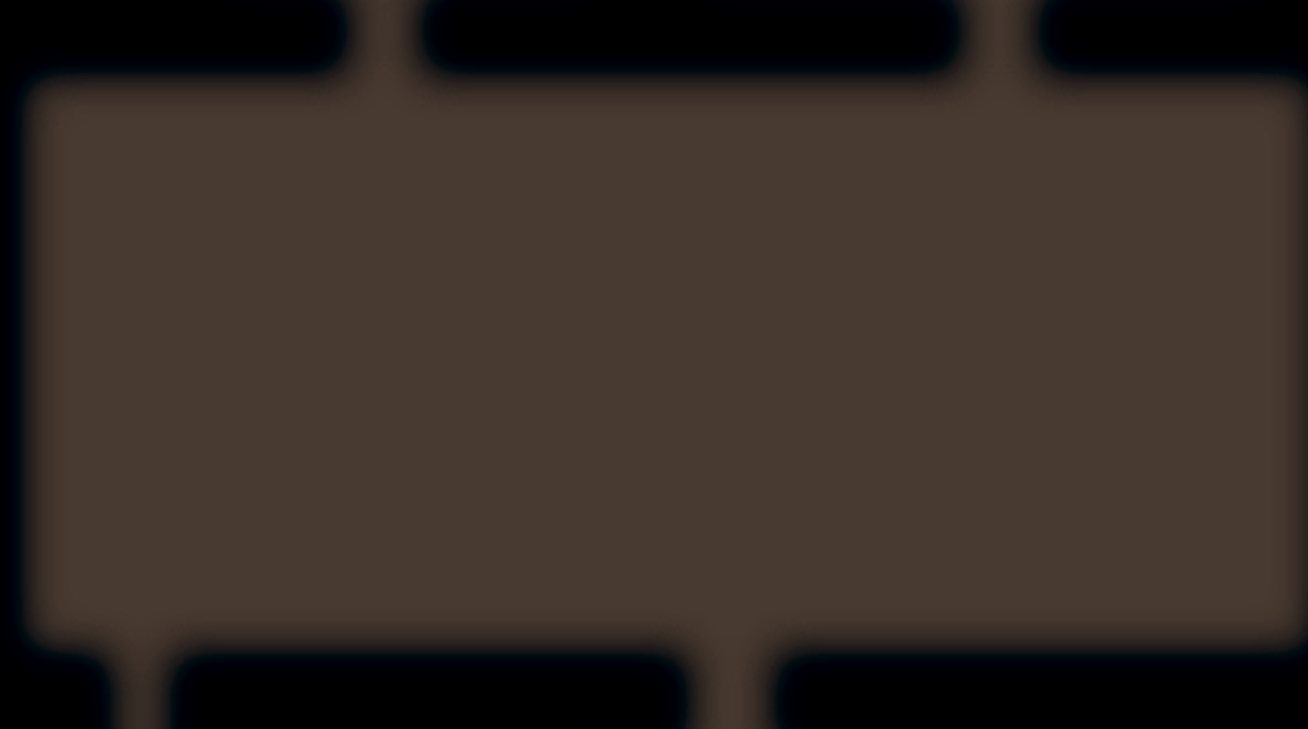
\includegraphics[scale=0.3]{images/nonPaused.png}
	\caption{nonPaused}
	\label{fig:nonPaused}
\end{figure}

\begin{figure}[!ht]
	\centering
	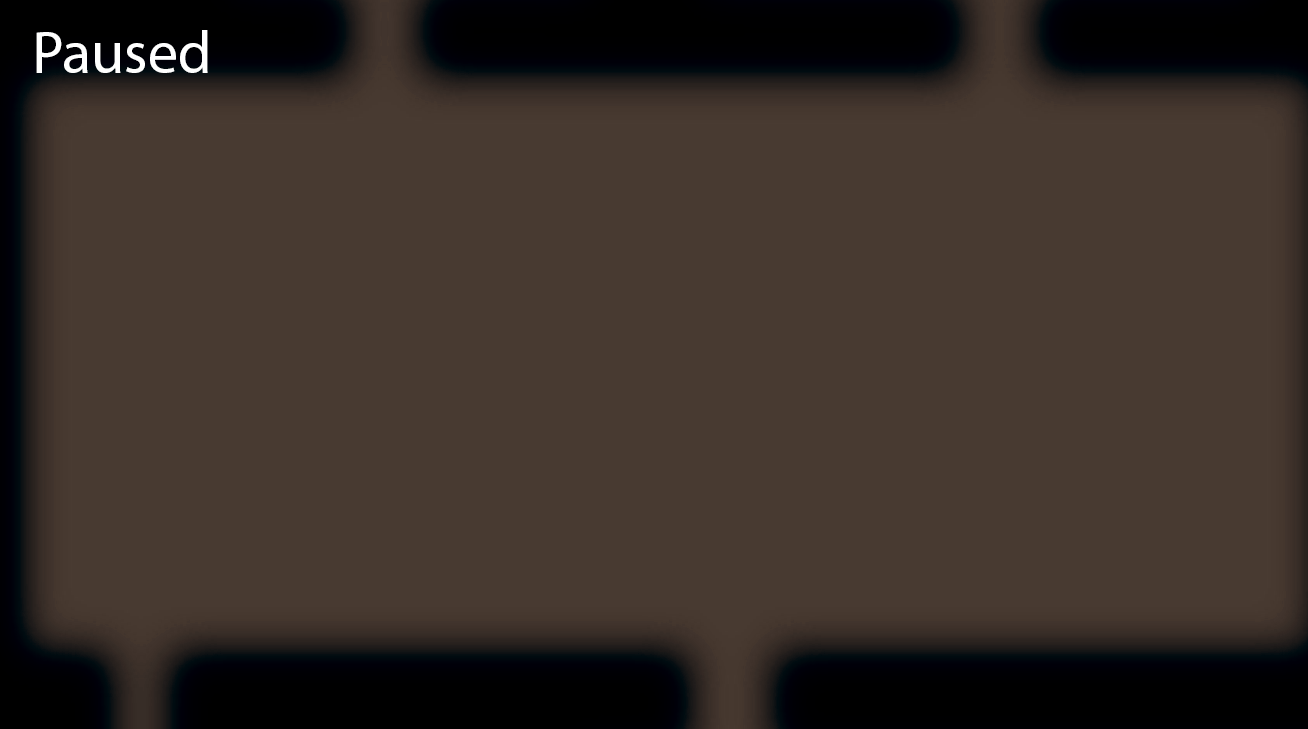
\includegraphics[scale=0.3]{images/Paused.png}
	\caption{Paused}
	\label{fig:Paused}
\end{figure}

\begin{figure}[!ht]
	\centering
	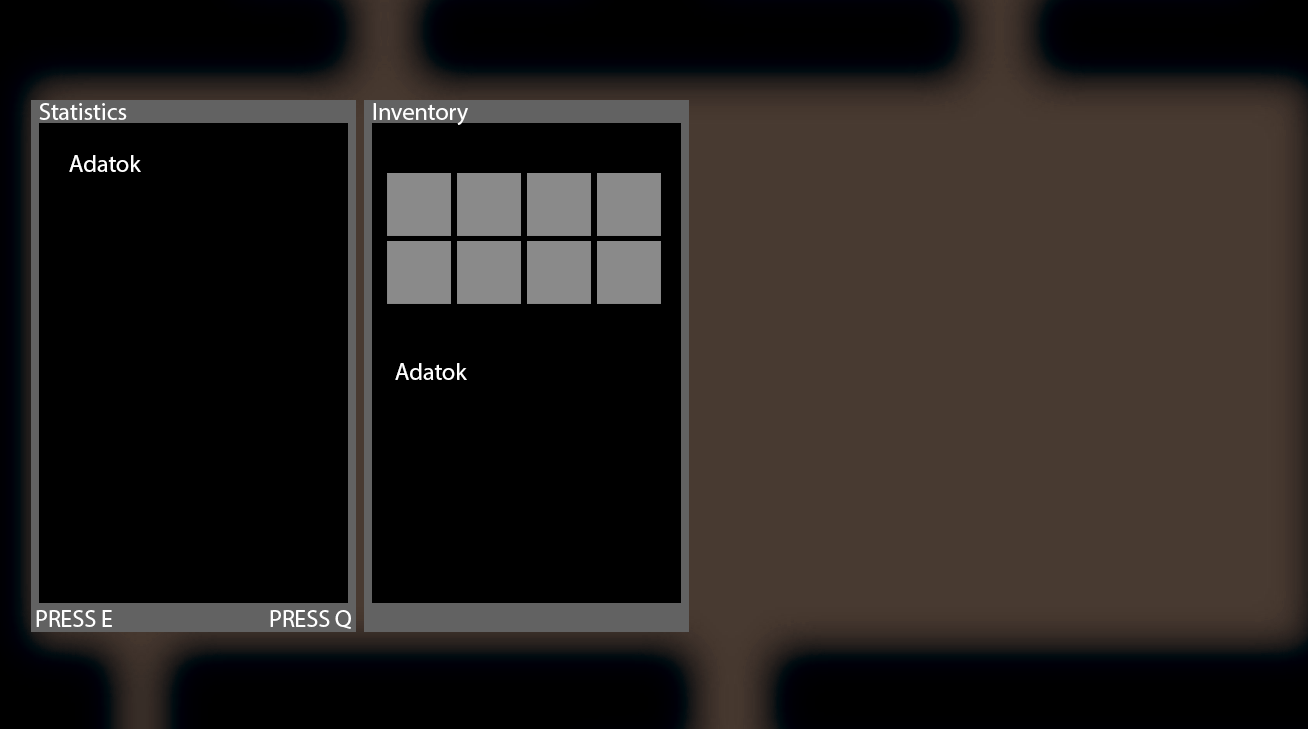
\includegraphics[scale=0.3]{images/Inventory.png}
	\caption{Inventory}
	\label{fig:Inventory}
\end{figure}

\begin{figure}[!ht]
	\centering
	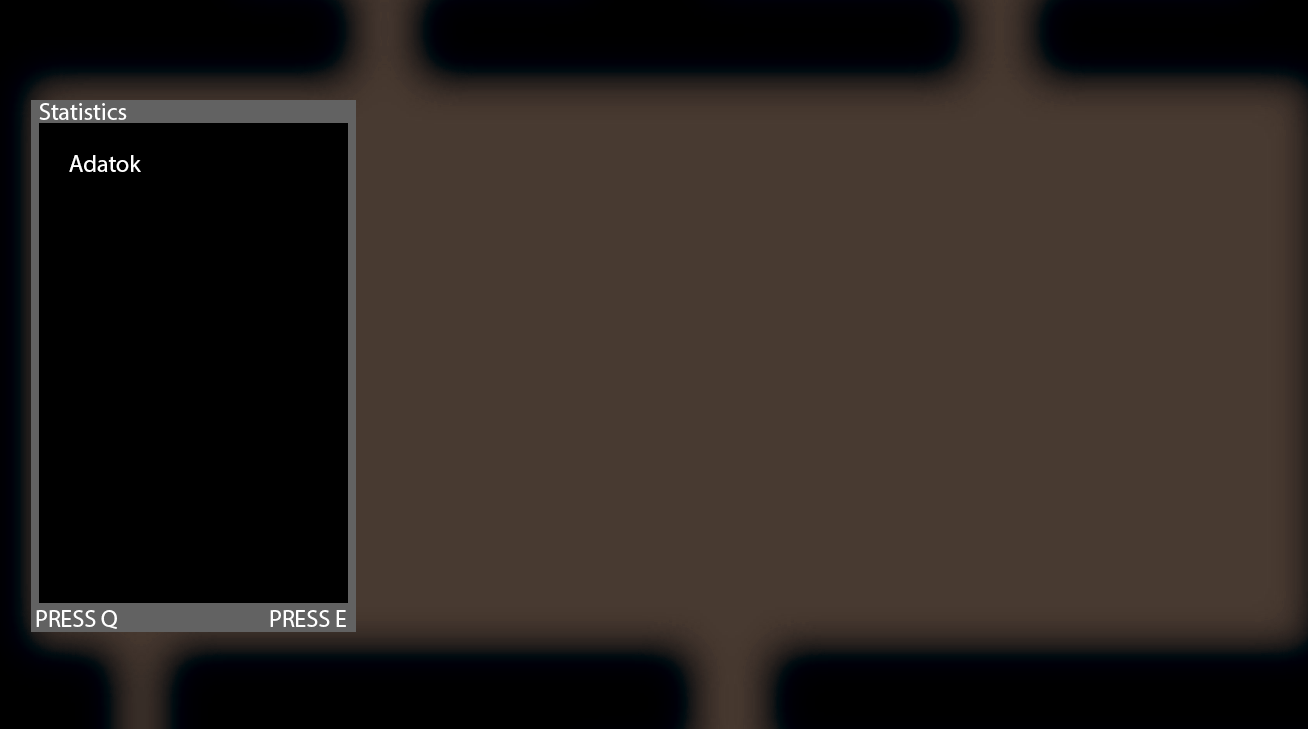
\includegraphics[scale=0.3]{images/Statistics.png}
	\caption{Statistics}
	\label{fig:Statistics}
\end{figure}

\begin{figure}[!ht]
	\centering
	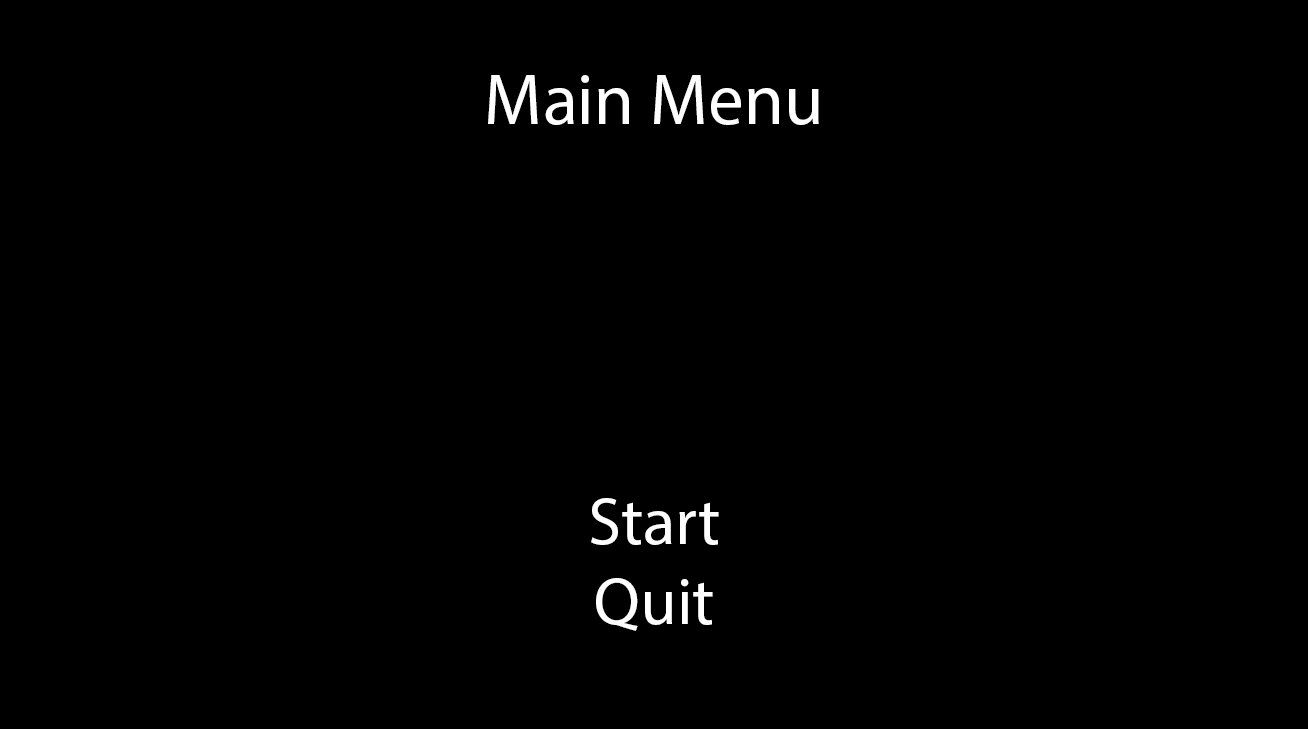
\includegraphics[scale=0.3]{images/MainMenu.png}
	\caption{Main Menu}
	\label{fig:MainMenu}
\end{figure}

\begin{figure}[!ht]
	\centering
	
\includegraphics[scale=0.3]{images/endscreenblue.png}
	\caption{Blue End Screen}
	\label{fig:BlueEndScreen}
\end{figure}

\begin{figure}[!ht]
	\centering
	
\includegraphics[scale=0.3]{images/endscreenred.png}
	\caption{Red End Screen}
	\label{fig:RedEndScreen}
\end{figure}

\begin{figure}[!ht]
	\centering
	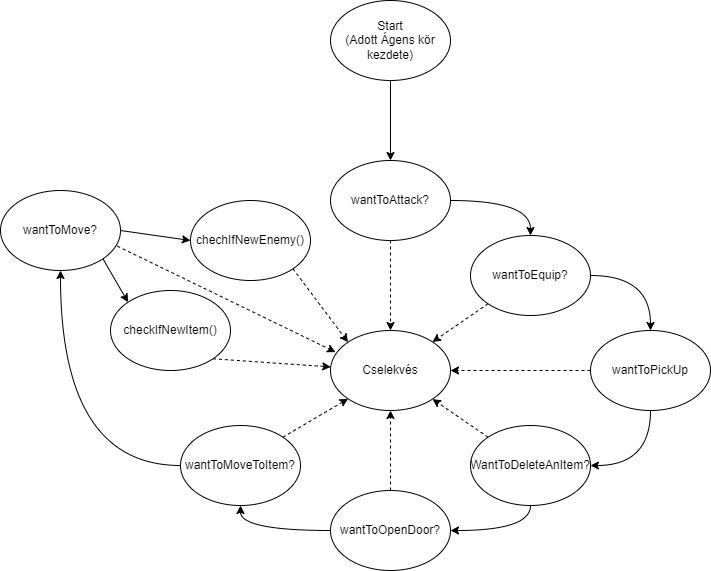
\includegraphics[scale=0.6]{images/agentfunction.png}
	\caption{Agent Action Priority}
	\label{fig:Priority}
\end{figure}

\begin{table}[h!]
    \begin{center}
    \begin{tabular}{ | c | c | c | }
    \hline
    
\includegraphics[width=0.3\textwidth, height=60mm]{images/Entity_Armor_01.png}
    & 
    
\includegraphics[width=0.3\textwidth, height=60mm]{images/Entity_Helmet_01.png}    
    & 
    
\includegraphics[width=0.3\textwidth, height=60mm]{images/Entity_Weapon_01.png}
    \\
    \hline
    
\includegraphics[width=0.3\textwidth, height=60mm]{images/Entity_Armor_02.png}
    & 
    
\includegraphics[width=0.3\textwidth, height=60mm]{images/Entity_Helmet_02.png}    
    & 
    
\includegraphics[width=0.3\textwidth, height=60mm]{images/Entity_Weapon_02.png}
    \\
    \hline
    \end{tabular}
    \caption{Item set 01}
    \label{tbl:Equipable items}
    \end{center}
\end{table}

\begin{table}[h!]
    \begin{center}
    \begin{tabular}{ | c | c | }
    \hline
    
\includegraphics[width=0.3\textwidth, height=60mm]{images/key.png}
    & 
    \includegraphics[width=0.3\textwidth, height=60mm]{images/Door.png}    
    \\
    \hline
    \end{tabular}
    \caption{Key and Door}
    \label{tbl:Key and Door}
    \end{center}
\end{table}

\begin{table}[h!]
    \begin{center}
    \begin{tabular}{ | c | c | c | }
    \hline
    
\includegraphics[width=0.3\textwidth, height=60mm]{images/block_brick.png}
    & 
    
\includegraphics[width=0.3\textwidth, height=60mm]{images/block_grass.png}    
    & 
    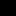
\includegraphics[width=0.3\textwidth, height=60mm]{images/block_empty.png}
    \\
    \hline
    \end{tabular}
    \caption{Blockok}
    \label{tbl:Blocks}
    \end{center}
\end{table}

\begin{table}[h!]
    \begin{center}
    \begin{tabular}{ | c | c | c | }
    \hline
    
\includegraphics[width=0.3\textwidth, height=60mm]{images/chest_0.png}
    & 
    
\includegraphics[width=0.3\textwidth, height=60mm]{images/chest_1.png}    
    & 
    
\includegraphics[width=0.3\textwidth, height=60mm]{images/object_brick.png}
    \\
    \hline
    \end{tabular}
    \caption{Chests and Brick}
    \label{tbl:Chests and Brick}
    \end{center}
\end{table}